\documentclass{article}
\title{Relatório 1\\ {\Large EEL7801}}
\author{Aluno: Carlos Freitas}
\date{28 de Setembro de 2023}
\setlength{\parindent}{4em}
\renewcommand{\figurename}{Figura}
\usepackage[letterpaper,top=3cm,bottom=3cm,left=3cm,right=3cm,heightrounded]{geometry}

\usepackage{graphicx}
\usepackage{indentfirst}
\graphicspath{{images/}}

\begin{document}

\maketitle

\section*{Desenvolvimento Geral}

O projeto é subdividido em 3 blocos, firmware, software e hardware, todas tiveram 
avanços em relação a proposta do projeto. As próximas seções terão foco no desenvolvimento
individual de cada bloco com mais detalhes. Em relação ao desenvolvimento geral do projeto
tem-se uma pequena mudança na estrutura do software, especificamente no servidor, tal mudança
se refere a exclusão do processamento de machine learning, tendo em seu lugar
um visualizador de dados, o qual permitiria a observação das medidas
coletados pelos sensores.

\section{Software}

O software é composto por dois blocos, a visualização dos dados e o servidor. 
Sendo a conexão entre o bloco embarcado e o "mundo de fora", bem como o responsável 
por armazenar os dados coletados, o servidor é a parte fundamental do software,
ele é feito na linguagem de programação Rust, linguagem que vem ganhando espaço 
no mercado web e de embarcados por sua segurança e performance. O código em si, utiliza
das "crates" axum, tokio e serde que permitem a criação de um servidor web 
assíncrono, de alta performance.
Além disso, o servidor utiliza a "crate" sqlx para a integração com o banco de dados, 
o qual é criado pela "engine" Sqlite, escrita em C e amplamente utilizada em ambientes
mais restritos como em um celular, tablet, etc.

\begin{figure}[ht]
	\centering
	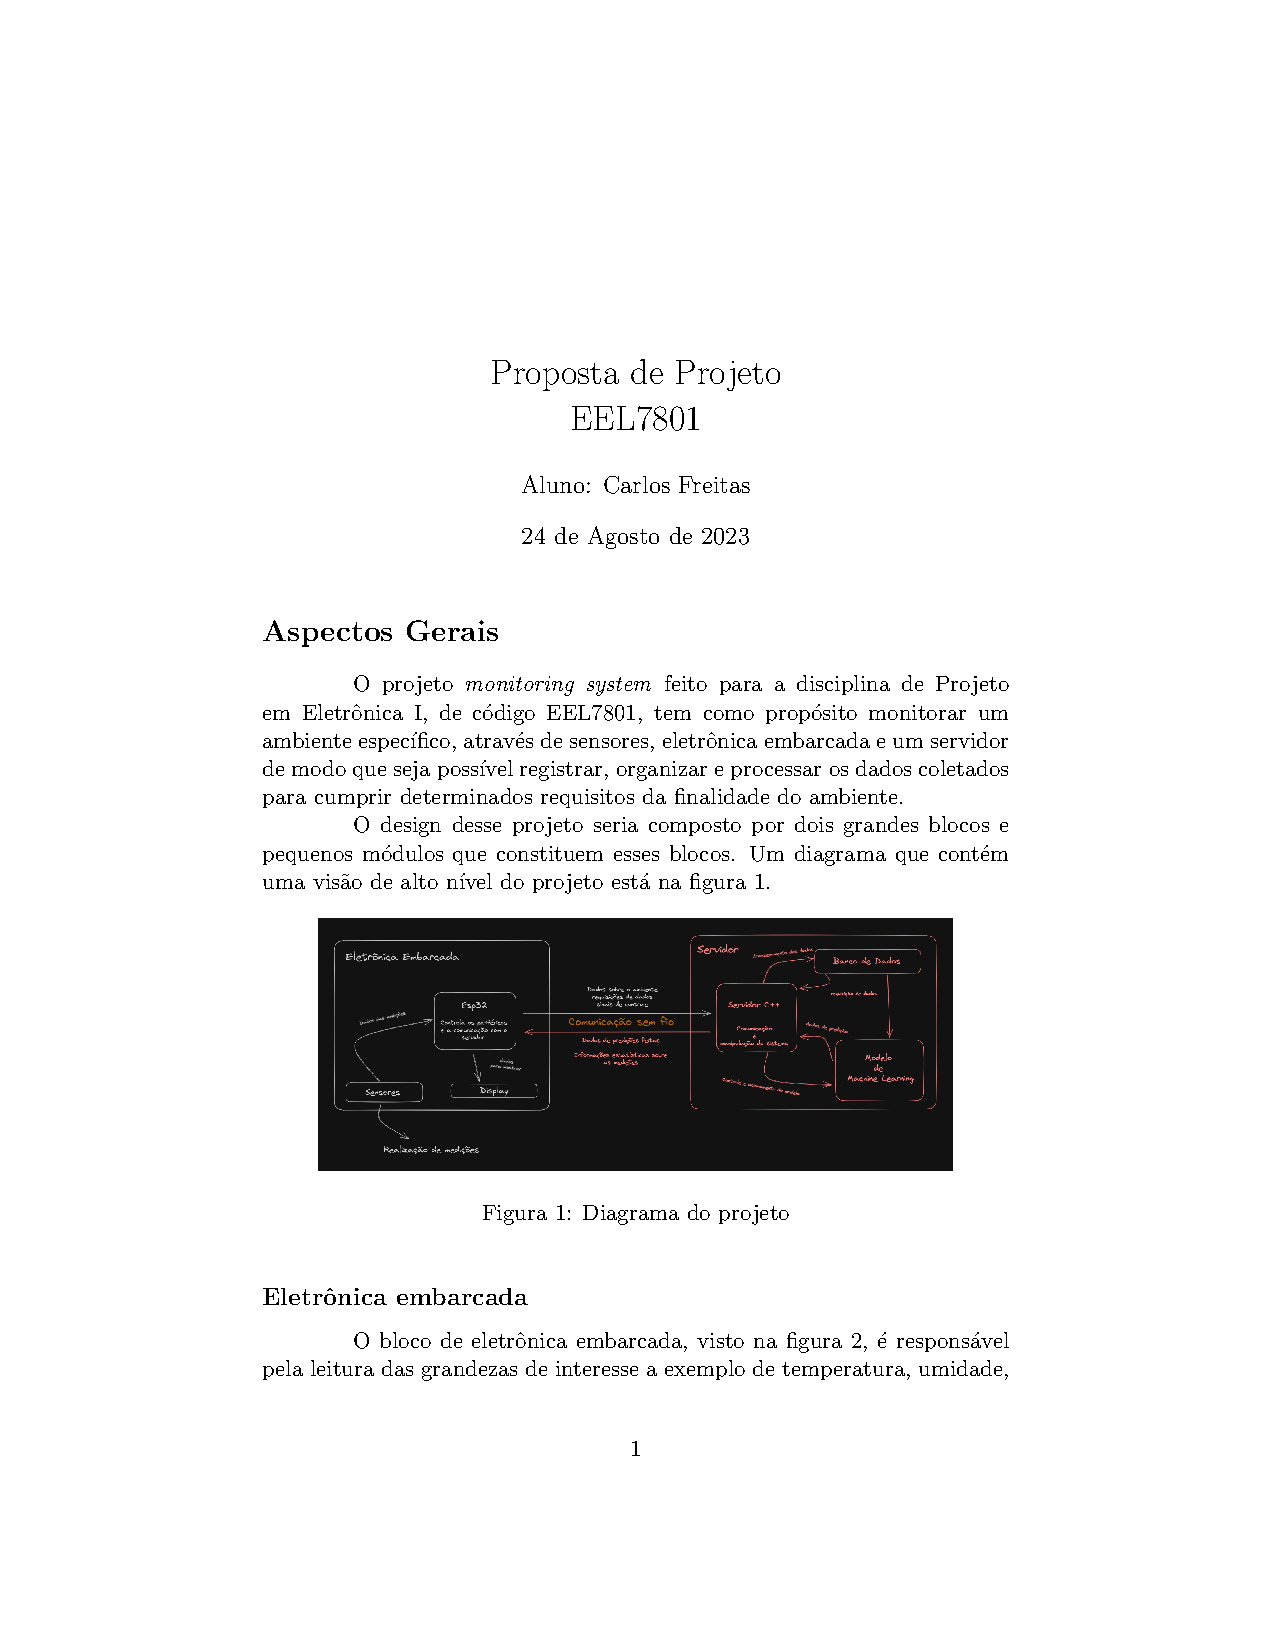
\includegraphics[width=0.85\textwidth,height=5cm,keepaspectratio]{main.jpg}
	\caption{Arquivo fonte "main" do servidor}
	\label{fig:main}
\end{figure}

Com o servidor estando ligado é preciso definir como ele cuidará das requisões 
enviadas para ele, as quais, nesse caso, seriam de envio de dados provenientes 
do esp32 e requisição de dados tanto pelo esp32 como por requisições externas.
Um esboço das funções que cuidam dessa função está presente na figura \ref{fig:handler}.
Nessa figura pode-se ver o protótipo de três dessas funções que manipulam as requisições
"get\_complete\_data\_handler", "post\_measuring\_handler"
e "get\_statistics\_handler", bem como três structs que representam as struturas das mensagens,
que teriam formato Json.

\begin{figure}[ht]
	\centering
	\includegraphics[width=0.95\textwidth,height=8cm,keepaspectratio]{handlers.png}
	\caption{Arquivo fonte que processa as requisições}
	\label{fig:handler}
\end{figure}

Quanto ao visualizador de dados, ele é um script feito com python para se 
emular uma requisição ao servidor e então utilizar os dados recebidos via http
para se traçar gráficos do comportamento das medidas de cada sensor. O andamento 
do script pode ser visto na figura \ref{fig:view}.

\begin{figure}[h]
	\centering
	\includegraphics[width=0.95\textwidth,height=5cm,keepaspectratio]{view.jpg}
	\caption{Arquivo fonte que processa as requisições}
	\label{fig:view}
\end{figure}

\section{Firmware}

O Firmware do projeto será feito integralmente no framework esp-idf da espressif, empresa 
responsável pelo esp32, usando C++ como linguagem de programação. Esse bloco do projeto será
responsável por coordenar a leitura dos sensores, o envio para o servidor e a visualização por meio
de um display. Nessa parte serão desenvolvidos drivers para o controle dos sensores e a interface 
da comunicação sem fio.

\begin{figure}[h]
	\centering
	\includegraphics[width=0.95\textwidth,height=5cm,keepaspectratio]{firmware1.jpg}
	\caption{Estrutura de arquivos do Firmware}
	\label{fig:firmware}
\end{figure}

\section{Hardware}

O Hardware é bastante simples, sendo composto por um esp32, dois sensores de temperatura, um lm35
e um dht11, que funciona também como sensor de humidade, além disso há também um sensor de irradiância
ultravioleta, gyml8511, e um sensor de qualidade do ar, cjmcu-811. Para visualização dos dados "localmente" tem-se  
um display.

Todos os dispositivos, display e sensores, serão gerenciados pelo esp32 levando em conta seus tempos 
de amostragem, formas de comunicação, etc. Infelizmente ainda não fiz o esquemático e realizei os 
testes físicos, pois nem todos os sensores foram entregues. No entanto, as conexões serão relativamente
simples, com pouca ou nenhuma adição além de resistores de pull-up e semelhantes, isso se deve a inclinação
da complexidade estar no software e firmware que manejariam a sincronia e a comunicação por código invés
de por hardware.



\end{document}

